\documentclass[10pt]{article}
% page setup
\usepackage[a4paper, total={6in, 8.75in}]{geometry}
\usepackage{parskip}
% formatting
\usepackage[utf8]{inputenc} % allow utf-8 input
\usepackage[T1]{fontenc} % use 8-bit T1 fonts
% cross-referencing
\usepackage{hyperref}
\usepackage{url}
\usepackage{doi}
% tables
\usepackage{booktabs}
% fonts
\usepackage{amsfonts}
\usepackage{microtype}
% s
\usepackage{graphicx}
\usepackage{float}
% math
\usepackage{amsmath}
% tables
\usepackage{tabularx}
\usepackage{colortbl}
% boxes
\usepackage{fancybox}
% tikz
\usepackage{tikz}
\usetikzlibrary{backgrounds}
\usetikzlibrary{arrows}
\usetikzlibrary{shapes,shapes.geometric,shapes.misc}
% landscape pages
\usepackage{pdflscape}
% chemical formulas
\usepackage{chemformula}
% smart references
\usepackage[capitalise, nameinlink]{cleveref}

\renewcommand{\thefigure}{SI\arabic{figure}}
\renewcommand{\thetable}{SI\arabic{table}}

% custom equation numbering
% https://tex.stackexchange.com/a/184641/
\newcounter{defcounter}
\setcounter{defcounter}{0}
\newenvironment{myequation}{%
\addtocounter{equation}{-1}
\refstepcounter{defcounter}
\renewcommand\theequation{SI\thedefcounter}
\begin{equation}}
{\end{equation}}

% this style is applied by default to any tikzpicture included via \tikzfig
\tikzstyle{tikzfig}=[baseline=-0.25em,scale=0.5]

% these are dummy properties used by TikZiT, but ignored by LaTex
\pgfkeys{/tikz/tikzit fill/.initial=0}
\pgfkeys{/tikz/tikzit draw/.initial=0}
\pgfkeys{/tikz/tikzit shape/.initial=0}
\pgfkeys{/tikz/tikzit category/.initial=0}

% standard layers used in .tikz files
\pgfdeclarelayer{edgelayer}
\pgfdeclarelayer{nodelayer}
\pgfsetlayers{background,edgelayer,nodelayer,main}

% style for blank nodes
\tikzstyle{none}=[inner sep=0mm]

% include a .tikz file
\newcommand{\tikzfig}[1]{%
{\tikzstyle{every picture}=[tikzfig]
\IfFileExists{#1.tikz}
  {\input{#1.tikz}}
  {%
    \IfFileExists{./figures/#1.tikz}
      {\input{./figures/#1.tikz}}
      {\tikz[baseline=-0.5em]{\node[draw=red,font=\color{red},fill=red!10!white] {\textit{#1}};}}%
  }}%
}

% the same as \tikzfig, but in a {center} environment
\newcommand{\ctikzfig}[1]{%
\begin{center}\rm
  \tikzfig{#1}
\end{center}}

% fix strange self-loops, which are PGF/TikZ default
\tikzstyle{every loop}=[]
%\documentclass[]{spie}  %>>> use for US letter paper
\documentclass[a4paper,nocompress]{spie}  %>>> use this instead for A4 paper
%\documentclass[nocompress]{spie}  %>>> to avoid compression of citations

\renewcommand{\baselinestretch}{1.0} % Change to 1.65 for double spacing
 
\usepackage{amsmath,amsfonts,amssymb}
\usepackage{graphicx}
\usepackage[colorlinks=true, allcolors=blue]{hyperref}
\usepackage[dvipsnames]{xcolor}
\usepackage{tabularx}
\setlength{\extrarowheight}{2pt}

\title{Quantifying the Impact \\ of Performance Improvements and Cost Reductions \\ from 20 years of Light-Emitting Diode Manufacturing}

\author[a,b]{Michael Weinold}
\author[b]{Sergey Kolesnikov}
\author[c]{Laura Diaz Anadon}
\affil[a]{ETH Zurich, Chair of Entrepreneurial Risks, Scheuchzerstrasse 7, 8092 Zurich, Switzerland}
\affil[b]{University of Cambridge, Centre for Environment, Energy and Natural Resource Governance, The David Attenborough Building, CB2 3QZ Cambridge, UK}

\authorinfo{Further author information: (Send correspondence to Michael Weinold)\\Michael Weinold: E-mail: michael.weinold@alumni.ethz.ch}

% Option to view page numbers
\pagestyle{empty} % change to \pagestyle{plain} for page numbers   
\setcounter{page}{301} % Set start page numbering at e.g. 301
 
\begin{document} 
\maketitle

\begin{abstract}
We collected historical data on device performance, technological breakthroughs and manufacturing innovation for phosphor-converted white light-emitting diodes for the past 20 years. We used this information to identify and quantify the principal sources of performance improvements in LED manufacturing. We found that in order to quantify the impact of single technological changes, it is necessary to analyse performance improvements the device sub-efficiency level. We further developed a bottom-up manufacturing cost model with process step resolution that captures improvements in throughput, yield and related costs of all relevant manufacturing steps, as well as economies of scale to analyse cost reductions and their sources. It covers progress from early manufacturing in 2003 to today. We found that larger wafer sizes have been largely responsible for cost reductions. We found that XXX well known XXX.

\end{abstract}

% Include a list of keywords after the abstract 
\keywords{light-emitting diodes, innovation, efficiency, cost}

\section{INTRODUCTION}
\label{sec:intro}  % \label{} allows reference to this section

\clearpage
\section{METRICS}

Data is readily available for metrics describing overall device performance. Luminous efficacy of devices as well as total flux per device can be extracted from datasheets, together with electrical device parameters. However, 

For instance, a highly cited and frequently updated metric is the total flux per package \cite{Liu2009}\cite{haitz2011solid}\cite{cho2017white}\cite{Fontoynont2018}. In combination with the cost per total flux, this visualization is sometimes referred to as \textit{"Haitz's Law"}, in reference to an early report on LED development by Haitz et al. \cite{haitz1999case}. However, while these metrics are often used to showcase technological progress in light-emitting diode design and manufacturing, they have limited significance XXX. Firstly, it is not desirable in all applications to increase the total flux per device beyond a certain point. Reasons for limiting the total flux per device may include lighting design considerations to reduce glare \cite{khan2015led}, device efficiency considerations to avoid electrical droop at high operating currents associated with high brightness \cite{Piprek2010} and economical considerations where multiple LED die in a single package can achieve the same brightness as a single high-brightness LED die. Secondly, even if one were to disregard these limitations, the total flux per device would only be a proxy for technological improvements in light-emitting diodes, if it was referring to single chips, instead of multi-chip paackages. 
Figure \ref{fig:haitz} shows an updated and expanded overview of best performing devices, both at the chip and package level, inspired by \textit{"Haitz's Law"}. It is evident that the historical improvement in total flux per package for single chips is not as pronounced as for multi-chip packages. While \textit{"Haitz's Law"} remains a popular visualization related to the progress in light-emitting diode design and manufacturing, care must be taken to consider its limitations.

\begin{figure} [ht]
    \begin{center}
        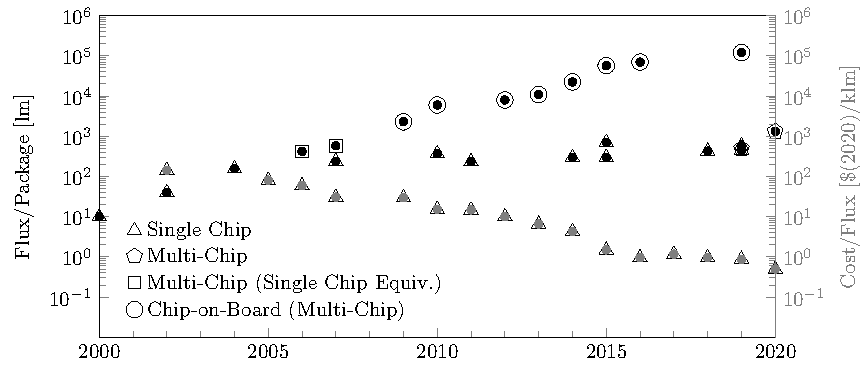
\includegraphics[width=\textwidth]{haitz_law_white.pdf}
    \end{center}
    \caption{Historical increase in flux for highest performing white light-emitting diode \underline{chips and (multi-chip) packages}, inspired by \textit{"Haitz's Law"}. Note that the increase in flux per single chip is not increasing as starkly as the flux for multi-chip packages. Shown are datapoints for best commercial performers from press releases, datasheets and and industry periodicals. Note the logarithmic ordinates and the black colored datapoints corresponding to the left ordinate, grey colored datapoints corresponding to the right ordinate. Sources: Data from Weinold et al. \cite{weinold2020technology}}
    \label{fig:haitz}
\end{figure}

Overall efficiency is cumulative from many sub-efficiencies caused by different physical effects \cite{schubert2018light}
In order to quantify the effect of single technological improvements on overall device performance, one must instead consider the metrics directly describing the various physical loss channels. Table \ref{tab:eff} lists the relevant sub-efficiencies considered along with mathematical definitions. The cumulative total lamp efficiency, defined as the product of all sub-efficiencies thus $\eta_L = \prod_{i=(V_f,\dots,S)} \eta_i$ XXX

The overall efficiency of a light-emitting diode is the product of the sub-efficiencies associated with an ensemble of different loss channels. Sub-efficiencies directly capture the effect of technology breakthroughs in device design and manufacturing process improvements. They thus provide the best metric to quantify technology breakthroughs.

Flicker \cite{weinold2020long}

        It describes the electrical and optical losses within the device, as well as the conversion losses in the phosphor layer. It further considers the mismatch between the device spectrum and an optimal spectrum, accounting for the wavelength dependent sensitivity of the human eye.

    \begin{table}[h!]
        \caption{List of the device sub-efficiencies used in our methodology. We follow the definitions used by previous authors, such as Tsao et al. \cite{tsao2010solid} and Pattison et al. \cite{pattison2017solid}. The historical development of the sub-efficiencies is displayed in figure \ref{fig:efficiency}. *Also called "lamp efficiency" or "cumulative efficiency" by authors, such as Tsao et al. \cite{tsao2010solid}}
        \bigskip
        \centering
    	\begin{tabularx}{\textwidth}{|l|l|l|X|}
    		\hline
    			\textit{Symbol} & \textit{Sub-Efficiency} & \textit{Loss-Channel} & \textit{Definition} \\
    		\hline
    		    $\eta_{V_f}$ & Forward Voltage Efficiency* & Ohmic Resistance & $\eta_{V_f} = E_{h\nu} / V_f $ \\
    		\hline
    		    $\eta_{LE}$ & Light-Extraction Efficiency & Re-absorption and Reflection & $\eta_{LE}= P_{out} / P_{in} $ \\
    		\hline
    		    $\eta_{IQ}$ & Internal Quantum Efficiency & Non-radiative Recombinations & $\eta_{EQ} = \eta_{IQ} \times \eta_{LE}$ \\
    		\hline
    		    $\eta_{Droop}$ & (Electrical) Droop & Non-radiative Recombinations & $\eta_{Droop} = 1 - \eta_{IQE} / \eta_{IQE}(A \rightarrow 0) $ \\
    		\hline
    		    $\eta_C$ & Conversion Efficiency & Stokes Loss, Absorption, etc. & $\eta_{C} = E_{\textcolor{blue}{B}} / \sum_{i=\textcolor{red}{R},\textcolor{orange}{O},\textcolor{yellow}{Y},\textcolor{teal}{G}} E_i$ \\
    		\hline
    		    $\eta_{S}$ & Spectral Efficiency & Eye Sensitivity & $\eta_{S} = K / K_{max}(CRI,CCT)$ \\
    		\hline
    		    $\eta_L$ & Lamp Efficiency & N/A (Cumulative) & $\eta_L = \prod_{i=(V_f,\dots,S)} \eta_i$ \\
            \hline
                \multicolumn{4}{|l|}{$\!\begin{aligned}
                    E_{h\nu} &\dots \text{photon energy} \\
                    V_f &\dots \text{forward voltage} \\
                    A &\dots \text{electrical current} \\
                    E_{B,\dots,G} &\dots \text{optical energy of monochromatic light (blue, red, orange, yellow, green)} \\
                    K &\dots \text{luminous efficacy of radiation} \\
                    CRI &\dots \text{color rendering index}, \ CCT \dots \text{color temperature} \\
                \end{aligned}$} \\
            \hline
    	\end{tabularx}
    	\label{tab:eff}
    \end{table}


\clearpage

\section{METHODS}
\label{sec:methods}

To quantify changes in the manufacturing cost of devices, a bottom-up manufacturing cost model with process step resolution was constructed to cover the entire manufacturing process of GaN-on-sapphire based phosphor converted low-to-mid power light-emitting diode packages of different chip architectures. We considered classical p-side-up lateral current spreading devices, as well as a packaged flip-chip vertical current spreading architecture and a chip-scale package flip chip architecture. The model was constructed for the years 2003, 2012 and 2020. It was populated with equipment data from European and North American firms, selected for a virtual North American manufacturing location. Process specific step parameters were derived from scientific literature, company publications, archived product catalogs and patent literature. Details of the manufacturing process, as well as changes in the same were gathered from detailed patent analysis, augmented by interviews with experts from industry and academia. For 2012, data for the model was adapted from the \textit{LEDCOM} cost model prepared for the US Department of Energy by Stephen Bland. The model includes both the wafer treatment process as well as the packaging process. It is important to note that the aim of the model is not to faithfully represent real world manufacturing conditions in Asia based plants, but rather to show the effect of single technological changes in the manufacturing process on total cost. This means that while the model does consider overhead costs and depreciation, it does so only to XXXX 

Also to diagreggate contribution of single changes
To dis-aggregate the contribution of changes in manufacturing process steps to total manufacturing cost, we used an approach introduced by Kavlak et al. in a cost model with similar process step resolution for solar photovoltaics. It is based on the logarithmic derivative of the total differential of the cost function.

The following discussion follows an approach developed by Kavlak et al. \cite{kavlak2018evaluating}. For the detailed derivation, we refer to this publication.

To gain a detailed understanding of the sources and magnitude of efficiency improvements in devices, we gathered data on overall device performance and identified the associated device architecture and types of down conversion phosphors used. We systematically identified the improvements related to each device sub-efficiency, gathered associated efficiency data from literature or computed the respective values from raw data.
For instance, in the case of spectral efficiency and the performance related to consumer experience metrics, we identified the prevalent red and yellow phosphors used during the period of interest. We then computed luminous efficacy of radiation as well as the color rendering index and color temperature from the spectral data. The development history of each phosphor was researched to determine if it had been developed specifically for use in light emitting devices, or if it was instead the result of a knowledge spillover.


figure: chip architectures
\begin{figure} [ht]
    \begin{center}
        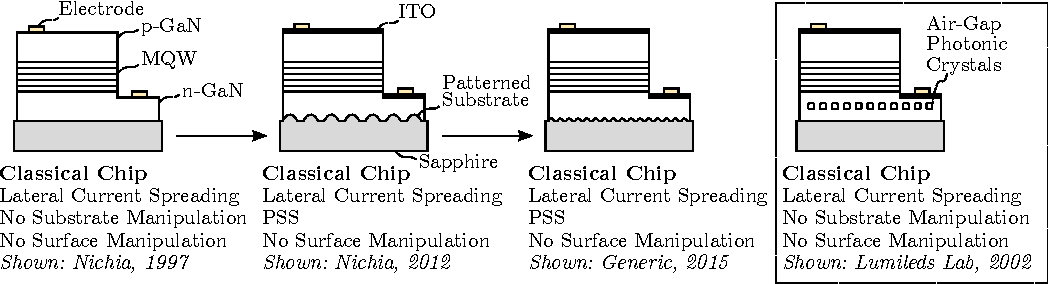
\includegraphics[width=\textwidth]{SPIE/article/chip_architectures.pdf}
    \end{center}
    \caption{Cutaway side views of the evolution of chip architectures for classical chip designs (lateral current spreading). Note that dimensions are not to scale and smaller features are greatly exaggerated for visibility. Years correspond to earliest identified patent priority date. Dashed boxes indicate chip designs not brought to large scale production. Adapted from patents \cite{nagahama2013nitride}\cite{tanaka2010semiconductor}\cite{wierer2006photonic}}
    \label{fig:chip_arch}
\end{figure}

\begin{figure} [ht]
    \begin{center}
        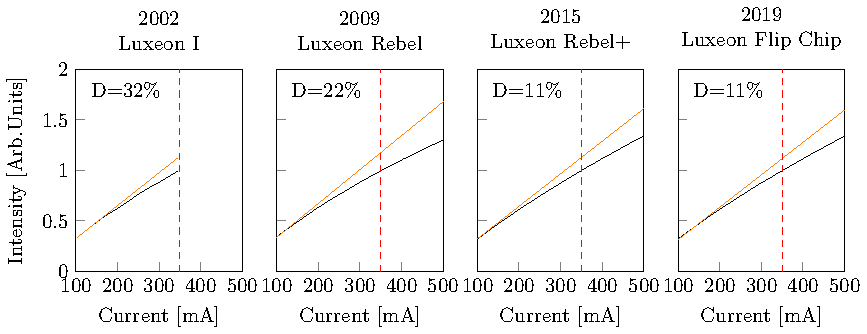
\includegraphics[width=0.85\textwidth]{SPIE/article/droop_lumileds.pdf}
    \end{center}
    \caption{Luminous intensity of four different \textit{Lumileds} high-power light-emitting diodes normalized to the value at a test current of $A_{test}=350$mA. The black curves describe the real measured intensity, the orange curves describe the estimated ideal intensity. Droop is the difference between these curves at the test current. Current-Intensity data extracted from device datasheets \cite{datasheet_lumileds_lux1}\cite{datasheet_lumileds_rebel}\cite{datasheet_lumileds_rebplus}\cite{lumi2019data}}
    \label{fig:chip_arch}
\end{figure}

\section{PERFORMANCE IMPROVEMENTS}

\begin{figure} [ht]
    \begin{center}
        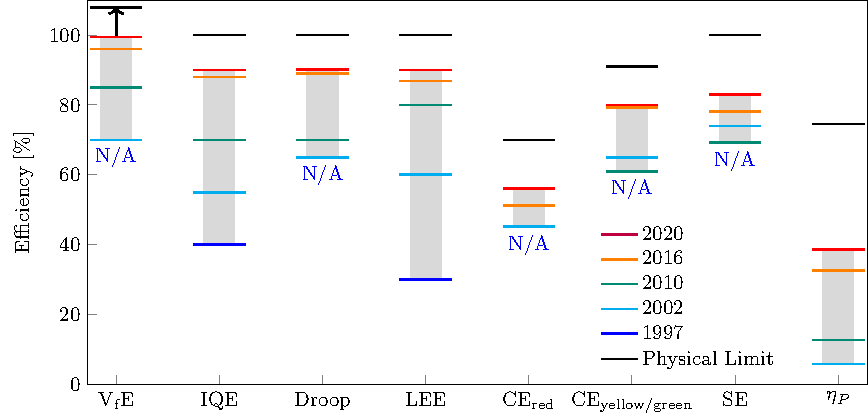
\includegraphics[width=0.85\textwidth]{SPIE/article/breakthroughs_efficiency.pdf}
    \end{center}
    \caption{Impact of technology breakthroughs and manufacturing process improvements on historical improvements in sub-efficiencies of phosphor-converted warm white light-emitting diodes with test currents of at least $I_\text{test}=350$mA. The overall lamp efficiency $\eta_L$ is displayed as the rightmost column. This figure takes as inputs the state-of-the-art sub-efficiencies discussed in section \ref{sec:methods}. Horizontal colored bars give state-of-the-art sub-efficiencies for five years: \textcolor{blue}{1997}, \textcolor{teal}{2002}, \textcolor{orange}{2010}, \textcolor{magenta}{2016} and \textcolor{red}{2020}. Colored annotation "N/A" indicates the sub-efficiency of the corresponding year cannot be computed for the following reasons: V$_\text{f}$E, Droop: depend on current, which was below 350mA at the time; CE, SE: warm white spectrum LEDs not available at the time. Physical limits are indicated by black horizontal bars. The possible range for the physical limit of V$_\text{f}$E exceeds 100\% and depends on electrical device parameters, which are discussed in \cite{david2016electrical}. The range is given by an upward pointing black arrow. Color of vertical bars indicates improvement through either technology spillovers or other improvements (technology breakthroughs or process learning). Spillovers are annotated and listed in an inset table. Efficiency acronyms: forward voltage efficiency (V$_\text{f}$E), internal quantum efficiency (IQE), light extraction efficiency (LEE), conversion efficiency (CE), spectral efficiency (SE), power conversion efficiency ($\eta_{PC}$). Spillover acronyms: patterned sapphire substrate (PSS), indium tin oxide (ITO). Sources: Data for sub efficiencies from \cite{weinold2020technology}}
    \label{fig:efficiency}
\end{figure}

\subsection{Physical Efficiency}

give two waterfall diagrams (2003,2020) and give one example
example: maybe droop with associated figure. is good example of process improvements

\subsection{Consumer Experience}

List phosphors, give a short overview but do not include figures
show cct spectrum with lines of YAG and 258+ phosphors

\section{MANUFACTURING COST}

show two waterfall diagrams (2003 only). mention work in progress



\clearpage
\acknowledgments % equivalent to \section*{ACKNOWLEDGMENTS}       
 
The main author gratefully acknowledged funding by the \textit{Swiss Study Foundation} of Zurich, Switzerland. The authors further gratefully acknowledge project funding by the \textit{Alfred P. Sloan Foundation} of New York, USA.

% References
\bibliography{report} % bibliography data in report.bib
\bibliographystyle{spiebib} % makes bibtex use spiebib.bst

\end{document} 


%%% custom definitions %%%%%%%%%%%%%%%%%%%%%%%%%%%%%%%%%%%%%%%%%%%%%%%%%%%%%%%%%%%%%%%%%

\definecolor{silver}{rgb}{0.75, 0.75, 0.75}

%%% document metadata %%%%%%%%%%%%%%%%%%%%%%%%%%%%%%%%%%%%%%%%%%%%%%%%%%%%%%%%%%%%%%%%%%

\title{Rapid technological progress in white light-emitting diodes \\ and its sources in innovation and technology spillovers  }
\date{February 2023}

\hypersetup{
    pdftitle={Supplementary Information},
    pdfauthor={Michael Weinold, Sergey Kolesnikov, Laura Diaz Anadon}
}

%%% document body %%%%%%%%%%%%%%%%%%%%%%%%%%%%%%%%%%%%%%%%%%%%%%%%%%%%%%%%%%%%%%%%%%%%%%%

\begin{document}

\setlength{\fboxsep}{10pt}
\fbox{
    \parbox{\textwidth}{
        \textbf{\textsc{Supplementary Information}} for: \\
        M. Weinold, S. Kolesnikov, L.D. Anadon \\
        "Rapid technological progress in white light-emitting diodes and its sources in innovation and technology spillovers" \textit{Energy and Environmental Science} (2023)
    }
}

\tableofcontents

\newpage

\section{Luminous Efficacy Metrics}

Figure 1 in the main publication uses luminous efficacy of radiation as the primary metric to describe progress in lighting technologies. Care must be taken not to confuse this metric with luminous efficacy of source, which is used in \ref{fig:phosphor_spectrum}.

\subsection{Luminous Efficacy of Radiation}
\label{subsec:ler}

This metric describes the match of a light-emitting diode package spectrum to the human visual system. Efficacy in lighting is dependent on the luminosity function, which describes the wavelength-dependent sensitivity of the human eye. A light source emitting very \textit{efficiently} in the infrared yet emitting no visible light has a very low \textit{efficacy}. The luminous efficacy of radiation $K$ is mathematically defined as the normalized, integrated product of the spectral radiant flux of a light source with the wavelength-dependent human sensitivity to light \cite{cie-term-effrad}

\begin{myequation}
\label{eqn:ler}
    K [\text{lm/W}_{opt}]= \frac{\int_0^\infty K( \lambda ) \phi \text{d} \lambda}{\int_0^\infty \phi \text{d} \lambda}
\end{myequation}

where

\begin{align*}
    K &\dots \text{spectral luminous efficacy} \\
    \phi &\dots \text{spectral radiant flux} \\
    \lambda &\dots \text{wavelength}
\end{align*}

This metric can be computed from spectral data alone and does not require additional spectral normalization. It enables straightforward comparison between the performance of different downconversion phosphors, as shown in the top panel of \cref{fig:phosphor_spectrum}. Light sources emitting in the far red or blue part of the spectrum have lower efficacy of radiation. Care must be taken not to confuse this efficacy metric with the \textit{efficacy of source} described in the following subsection.

\subsection{Luminous Efficacy of Source}
\label{subsec:les}

The luminous efficacy \textit{of a light source} $\eta$ is defined as the ratio between the emitted luminous flux and the consumed electrical power \cite{cie-term-effsrc}

\begin{myequation}
    \eta [\text{lm/W}_{el}]= \frac{\phi}{P_{el}}
\end{myequation}

This metric is often cited in device datasheets, scientific literature and textbooks when describing the performance of light-emitting diodes. Care must be taken not to confuse this efficacy metric with the \textit{luminous efficacy of radiation}, which depends only on the spectral characteristics of a light source. As the luminous efficacy of a light source $\eta$ captures the overall device efficacy, it depends on a large number of other device properties and parameters. This makes attribution of changes in this metric to individual changes in device design or manufacturing difficult. For this reason, we do not use this metric in our study.

\newpage
\section{Manufacturing Cost Model}
\label{sec:costmodel}

\subsection{Structure of the Model}

\begin{figure}[h!]
    \centering
    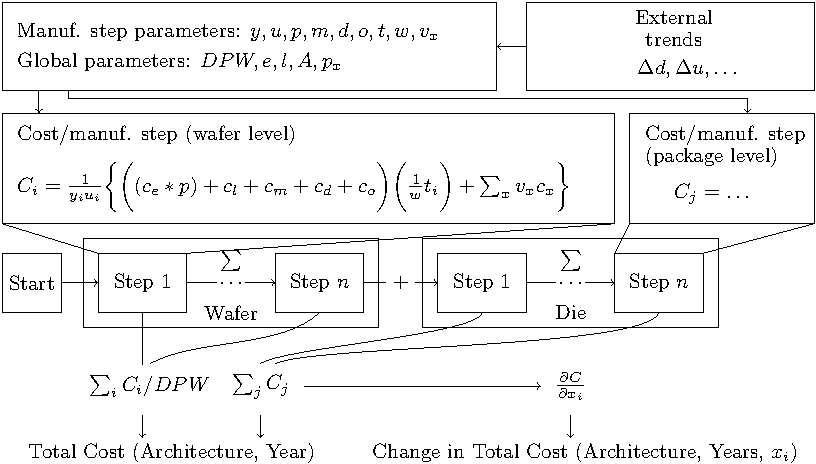
\includegraphics[width=0.95\textwidth]{./figures/cost_model.pdf}
    \caption{Schematic diagram of the cost model showing inputs to each step and computational steps leading to the cost model outputs. For the description of cost variables, see definitions for \cref{eqn:cost_wafer}.}
    \label{fig:costmodel-schematic}
\end{figure}

The cost model adapted for this publication is a microeconomic manufacturing cost model. Within the timeframe and scope laid out in the main publication, it returns the total manufacturing cost of phosphor converted warm white light-emitting diode packages. In this computation, it considers the main economic factors associated with operating and maintaining manufacturing equipment. It does not consider costs associated with research and development or those associated with the construction of manufacturing facilities. It considers market trends through their effect on manufacturing parameters.

A schematic diagram of the cost model is presented in \cref{fig:costmodel-schematic}. The cost model is process step-based. It is split between the two stages of the manufacturing process: the first stage combining operations at the wafer level, followed by the LED packaging stage. The model takes as inputs parameters specific to individual manufacturing process steps (\textit{"manufacturing step parameters"}) and parameters affecting all manufacturing steps (\textit{"global parameters"}). The cost for each process step is then computed. The cost model returns returns the costs of individual manufacturing steps as well as the total manufacturing cost. It further considers the yield per step and returns the cumulative yield, the yielded cost per step and the yielded total manufacturing cost.

\subsection{Manufacturing Process Steps by Chip Architecture}

\cref{fig:manuf_classical_2003}-\cref{fig:manuf_csp_2020-2} show a simplified rendering of the manufacturing process of three different chip architectures considered in the cost model.

    %CLASSICAL CHIP

    \begin{landscape}
        \begin{figure}
            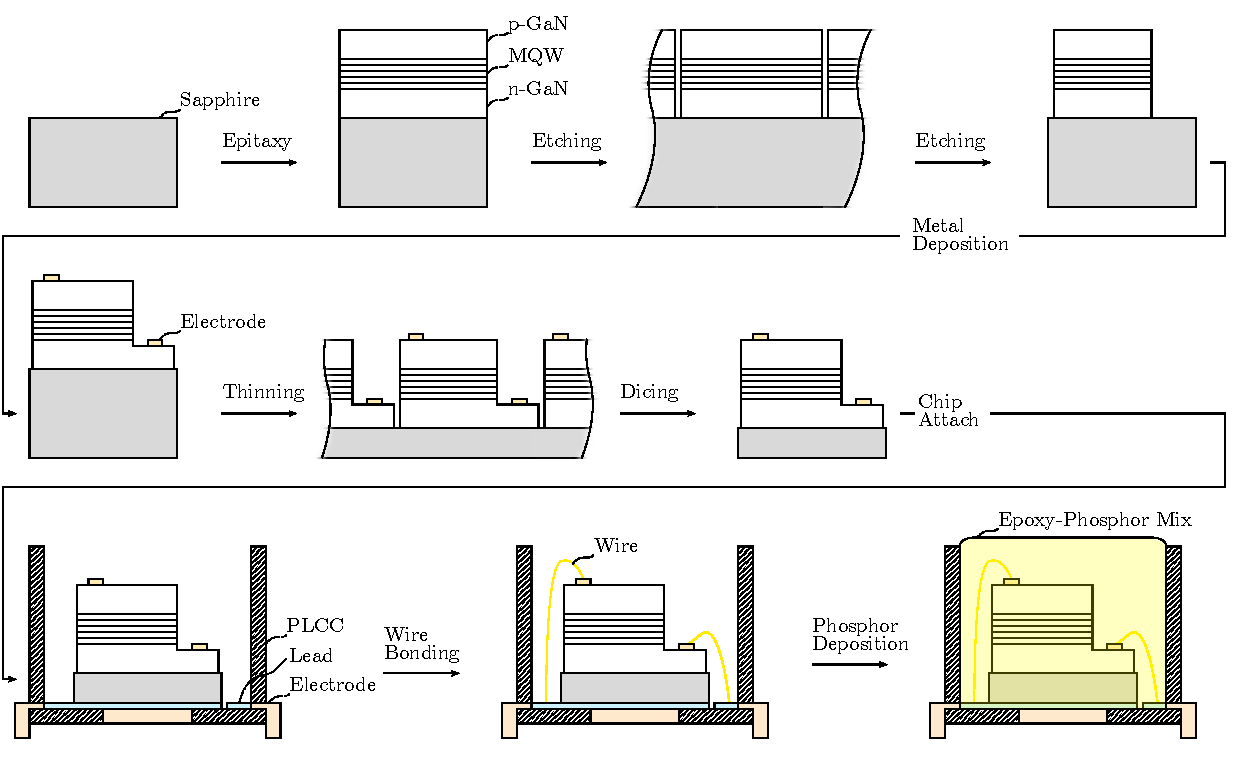
\includegraphics[width=555pt]{./figures/classical_overview_2003.pdf}
            \caption{Manufacturing process for a classical LED package with lateral current spreading, circa 2003. Abbreviations: MQW - multiple quantum well; PLLC - plastic leaded chip carrier.}
            \label{fig:manuf_classical_2003}
        \end{figure}
    \end{landscape}
    
    %VERTICAL THIN-FILM FLIP-CHIP

    \begin{landscape}
        \begin{figure}
            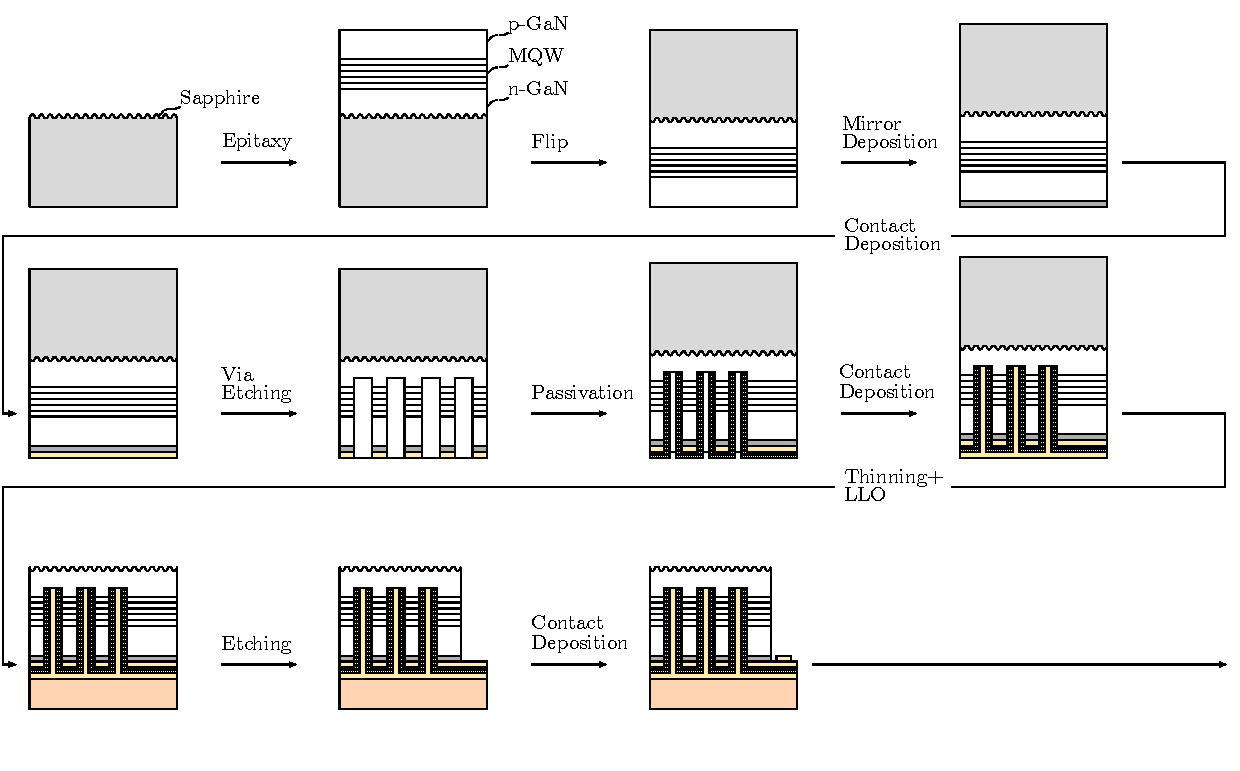
\includegraphics[width=595pt]{./figures/vtf_overview_2012-1.pdf}
            \caption{(1/2) Manufacturing process for a vertical thin-film  package flip-chip LED chip with vertical current spreading, circa 2012. Abbreviations: MQW - multiple quantum well; LLO - laser lift-off. Continued on next page.}
            \label{fig:manuf_vtf_2012-1}
        \end{figure}
    \end{landscape}

    \begin{landscape}
        \begin{figure}
            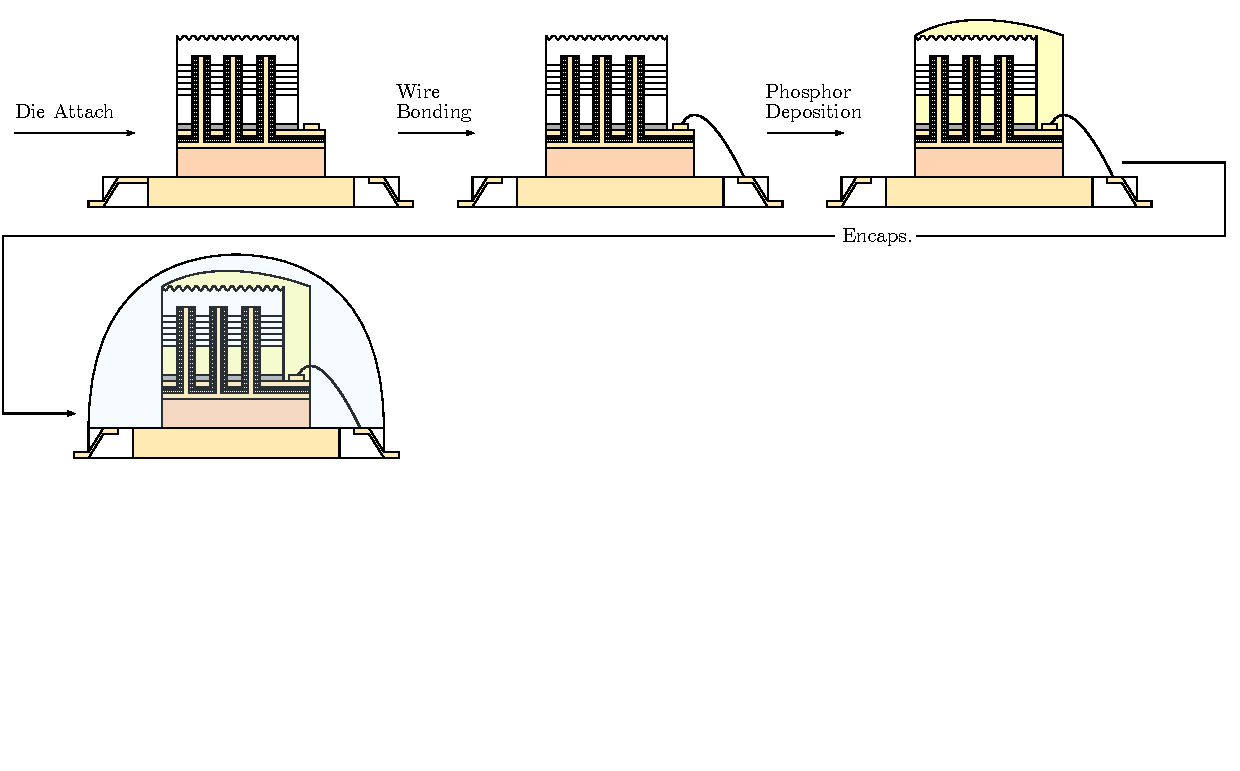
\includegraphics[width=595pt]{./figures/vtf_overview_2012-2.pdf}
            \caption{(2/2) Continued from previous page. Abbreviations: Encaps. - encapsulation.}
            \label{fig:manuf_vtf_2012-2}
        \end{figure}
    \end{landscape}

    % CHIP-SCALE PACKAGE FLIP-CHIP

    \begin{landscape}
        \begin{figure}
            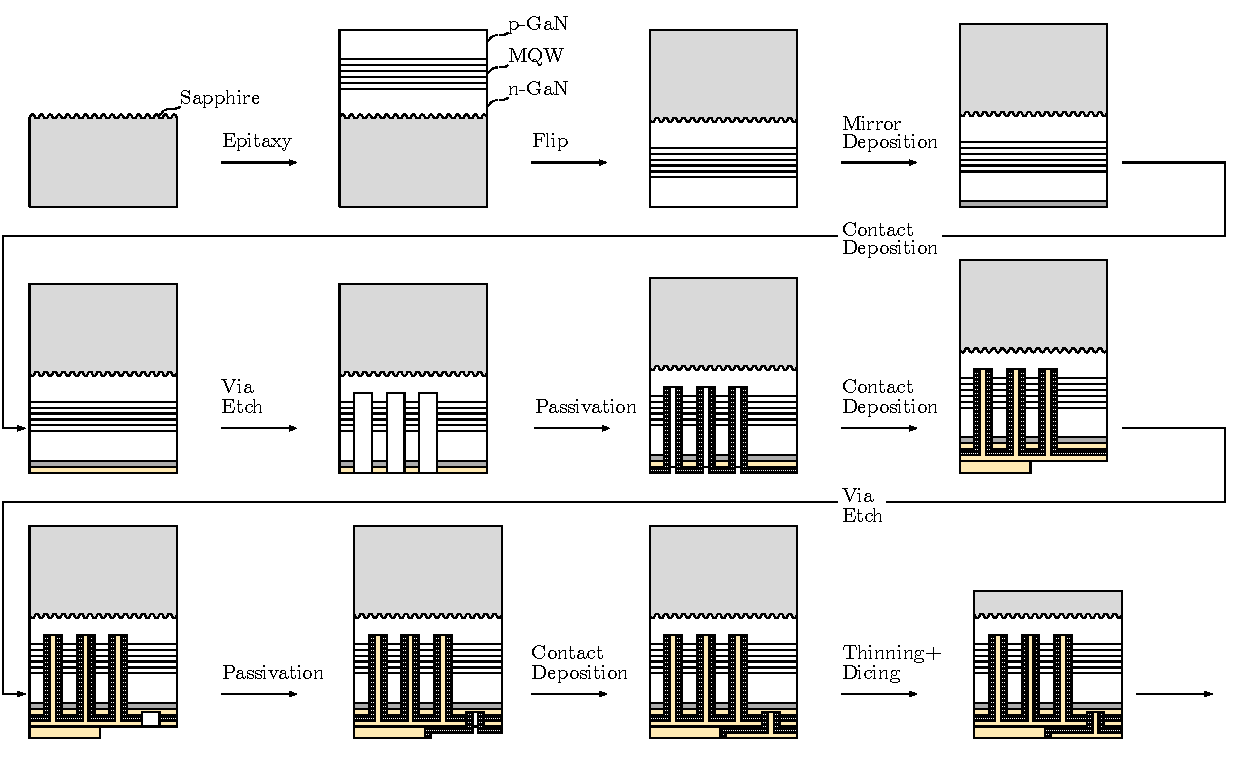
\includegraphics[width=595pt]{./figures/csp_overview_2020-1.pdf}
            \caption{(1/2) Manufacturing process for a chip scale package flip-chip LED chip with vertical current spreading, circa 2020. Abbreviations: MQW - multiple quantum well. Continued on next page.}
            \label{fig:manuf_csp_2020-1}
        \end{figure}
    \end{landscape}

    \begin{landscape}
        \begin{figure}
            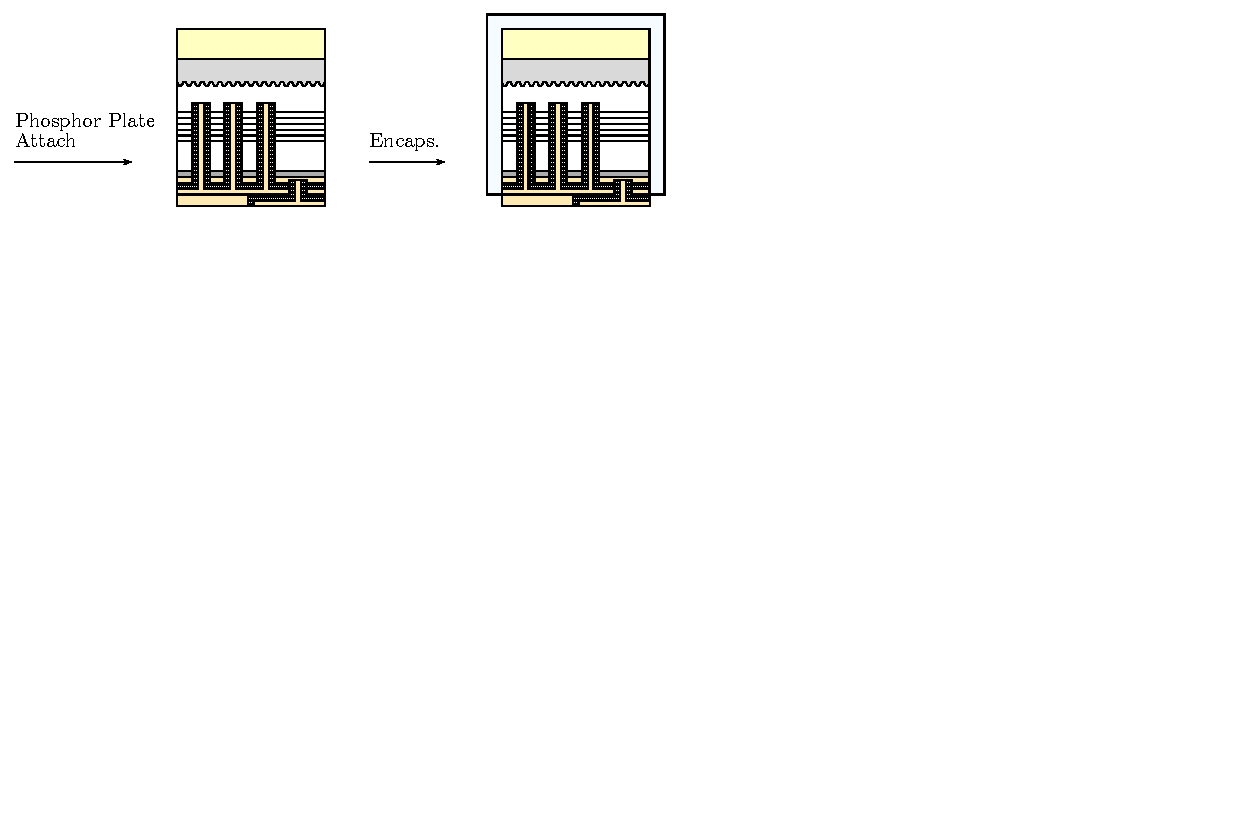
\includegraphics[width=595pt]{./figures/csp_overview_2020-2.pdf}
            \caption{(2/2) Manufacturing process for a chip scale package flip-chip LED chip with vertical current spreading, circa 2020. Continued from previous page. Abbreviations: Encaps. - encapsulation.}
            \label{fig:manuf_csp_2020-2}
        \end{figure}
    \end{landscape}

\subsection{Computation of Manufacturing Cost}

The manufacturing process of semiconductor devices can be categorized by the level at which manufacturing process steps are implemented, i.e., either at the wafer level or at the individual chip/package level. The total manufacturing cost per die is thus the sum of the total costs of all wafer processing steps and all die packaging steps.

\begin{myequation}
\label{eqn:cost_sum}
    C \bigg[ \frac{ \text{USD}(2020) }{ \text{die} } \bigg] = P_S + C_w + C_p
\end{myequation}

where

\begin{align*}
    P_S &\dots \text{sapphire substrate price per die} \\
    C_w &\dots \text{wafer processing cost per die} \\
    C_p &\dots \text{die processing cost}
\end{align*}

The total wafer processing cost and total die packaging costs are in turn the sum of all associated process steps.

\begin{myequation}
        C_w = \sum_i C_i
\end{myequation}
\begin{myequation}
	C_p = \sum_j C_j
\end{myequation}

The cost of a single process step $C_i$ can now be written as

\begin{myequation}
\label{eqn:cost_wafer}
    C_i \bigg[ \frac{ \text{USD}(2020) }{ \text{die} } \bigg] =\frac{1}{D}  \frac{1}{y_i}   \bigg\{ \bigg((c_e*p) + c_l + c_m + c_d + c_o \bigg)_i \bigg( \frac{t_i}{w_i u_i} \bigg) + \sum_{x} v_x \c_x \bigg\}
\end{myequation}

where the index $i$ runs over all wafer processing steps, the index $j$ runs over all die processing steps and the index $x$ run over all materials.

\begin{align*}
        D &\dots \text{number of functional (i.e., successfully tested) die per wafer}\\
        y &\dots \text{process step yield} \\
        u &\dots \text{equipment utilization (relative to theoretical equipment capacity)} \\
        p &\dots \text{power consumption} \\
        c_e &\dots \text{hourly electricity cost} \\
        c_m &\dots \text{hourly maintenance cost} \\
        c_d &\dots \text{hourly depreciation cost}\\
        c_l &\dots \text{hourly labour cost} \\
        c_o &\dots \text{hourly overhead cost} \\
        t_i &\dots \text{time per run} \\
        w &\dots \text{wafers per run} \\
        A &\dots \text{wafer area} \\
        v_x &\dots \text{volume of material $x$ per wafer} \\
        c_x &\dots \text{cost of material $x$ per volume}\\
\end{align*}

The number of die per wafer $D$ depends on the total usable wafer area. The usable area depends on the wafer diameter, the cutting street width between the chips and the exclusion zone at the rim of the wafer.

\begin{myequation}
	A_{\text{usable}}=A_{\text{wafer}}-A_{\text{cut}}-A_{\text{exclusion}}
\end{myequation}

Determining the usable wafer area as a function of these three parameters requires a numerical solution. However, following discussions in the literature \cite{de2005investigation}, we approximate the number of functional die per wafer\footnote{often \textit{"good die per wafer"} in the literature} as

\begin{myequation}
\label{eqn:dpw}
	DPW = \frac{\pi}{4}  \bigg ( \frac{d-2e}{\sqrt{a}+s/2} \bigg ) ^2 - \frac{\pi}{\sqrt{2}}\frac{d-2e}{(\sqrt{a}+s/2)^2}
\end{myequation}

where

\begin{align*}
    d &\dots \text{wafer diameter} \\
    e &\dots \text{wafer edge exclusion zone width} \\
    a &\dots \text{die area} \\
    s &\dots \text{cutting street width} \\
\end{align*}

\begin{figure}[h!]
    \centering
    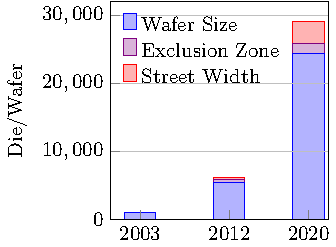
\includegraphics[width=5.5cm]{./figures/die-per-wafer.pdf}
    \caption{Number of die per wafer for the different wafer sizes used in different years: (DPW) $d(2002)=50$mm$\rightarrow851$DPW, $d(2002)=50$mm$\rightarrow5370$DPW, $d(2020)=100$mm$, \rightarrow26,838$DPW. Source: own estimates, based on \cref{eqn:dpw} and the dominant wafer size of the considered year, according to \cref{fig:wafers}.}
    \label{fig:dpw}
\end{figure}

Results are plotted in \cref{fig:dpw}, showing the increase in die per wafer (DPW) over time. \cref{eqn:dpw} then gives us for the cost of a manufacturing step $C_i$ in the wafer processing category
\begin{myequation}
\label{eqn:cost_wafer_full}
\begin{split}
    C_i \bigg[ \frac{ \text{USD}(2020) }{ \text{die} } \bigg] &= \bigg (  \frac{\pi}{4}  \bigg ( \frac{d-2e}{\sqrt{a}+s/2} \bigg ) ^2 - \frac{\pi}{\sqrt{2}}\frac{d-2e}{(\sqrt{a}+s/2)^2} \bigg )^{-1} \times \\
    &  \frac{1}{y_i}  \bigg\{ \bigg((c_e*p) + c_l + c_m + c_d + c_o \bigg)_i \bigg( \frac{t_i}{w_i u_i} \bigg) + \sum_{x} v_x \c_x \bigg\}
\end{split}
\end{myequation}
and the cost of a manufacturing step $C_j$ in the packaging category
\begin{myequation}
\label{eqn:cost_die}
    C_j \bigg[ \frac{ \text{USD}(2020) }{ \text{die} } \bigg] = \frac{1}{y_j}  \bigg\{ \bigg((c_e*p) + c_l + c_m + c_d + c_o \bigg)_i  \frac{c_j}{u_j} + \sum_{x} a v_x c_x \bigg\}
\end{myequation}
where $c_j$ is $\text{throughput}^{-1}$. The total cost is thus
\begin{myequation}
\label{eqn:cost_total}
\begin{split}
    C= P_s &+ \sum_i \bigg \{ \frac{1}{D} \frac{1}{y_i} \bigg[ \frac{t_i}{w_i u_i} \bigg((e*p) + l + m + d +o \bigg)_i  + \sum_{x} v_x p_x \bigg] \bigg \} + \\
    & + \sum_j \bigg \{ \frac{1}{y_j} \bigg[ \frac{c_j}{u_j}  \bigg((e*p) + l + m + d + o \bigg)_i + \sum_{x} a v_x p_x \bigg ] \bigg\}
\end{split}
\end{myequation}
Note that in keeping with the categorization introduced by the United States Department of Energy (cf. eg. \cite{doe_ssl_rnd_2019}), certain steps from these two categories are reported separately. In the wafer processing category, the epitaxy step is reported separately due to its complexity and the large share of cost carried. In the wafer processing category, the phosphor step is reported separately.

\subsection{Computation of Yielded Cost}

Devices may be damaged or otherwise rendered unusable during the manufacturing process. The ratio between the number of good devices per step and the number of handled devices per step is known as the yield. Optimizing this yield is critical for reducing manufacturing cost \cite{Kumar2006}. This is because cumulative yield quickly drops as the yield from manufacturing steps with below 100\% yield is multiplied. We must thus consider not only the manufacturing cost per process step, but also the cost including the yield \cite{becker2001use}\cite{becker2001using}. While there are different mathematical approaches to including yield, we follow the definition in \cite{becker2001use}. We write for the yielded cost $C_{Y_i}$ of a step $i$ with associated cost (before considering yield) $C_1$ and yield $Y_1$:

\begin{myequation}
\label{eqn:C_2}
    C_{Y_1} = \frac{C_1}{Y_1}
\end{myequation}
\begin{myequation}
    C_{Y_2} = \frac{C_1 + C_2}{Y_1 Y_2} - C_{Y_1} = \frac{C_1 + C_2}{Y_1 Y_2} - \frac{C_1}{Y_1} = \frac{1}{Y_1 Y_2} \bigg ( C_1 (1-Y_2) +C_2 \bigg)
\end{myequation}
\begin{myequation}
    C_{Y_i} = \frac{ \sum_{x \leq i} C_x }{ \prod_{x \leq i} Y_x } - \frac{ \sum_{x<i} C_x }{ \prod_{x<i} Y_x }
\end{myequation}

If a step is applied more than once, we can conveniently rewrite this in a form suited to computation within the \textit{Excel} worksheet. Assuming step $2$ is used twice, we get for the yielded cost of this step an equation of the form

\begin{myequation}
\label{eqn:C_2^2}
    C_{Y_2}^{(2 \times)} = \bigg( \frac{C_1 + C_2}{Y_1 Y_2} - \frac{C_1}{Y_1} \bigg) + \bigg( \frac{C_1 + 2 C_2}{Y_1 Y_2^2} - \frac{C_1 + C_2}{Y_1 Y_2}     \bigg)
\end{myequation}
\begin{myequation}
    = \frac{1}{Y_1 Y_2^2} \bigg( C_1 (1-Y_2^2) +2C_2 \bigg)
\end{myequation}

which can be compared to  \cref{eqn:C_2} to find a more general form:

\begin{myequation}
    C_{Y_2}^{(n \times)} = \frac{1}{Y_1 Y_2^n} \bigg( C_1 (1-Y_2^n)+nC_2\bigg)
\end{myequation}

It can be shown by induction that the general form of a term for a step $i>1$ repeated $n$ times can be expressed as:

\begin{myequation}
\label{eqn:yielded_cost}
    C_{Y_{i>1}}^{(n \times)} = \frac{1}{Y_i^{n-1} \prod_{x \leq i} Y_x} \bigg( nC_i + \sum_{x < i} C_x (1-Y_i^n) \bigg)
\end{myequation}

This cumulative approach to yielded cost is different from the approach taken in the original \textit{LEDCOM} model. It uses what in the literature is described as an \textit{"itemized approach"} to yielded cost \cite{becker2001use}. In this approach, the yielded cost of a single process step $f$ is described as

\begin{myequation}
	f_\text{single} = \frac{i+s}{y}
\end{myequation}

where

\begin{align*}
    i &\dots \text{material cost of previous step} \\
    s &\dots \text{step cost}
\end{align*}

For process steps that are performed more than once, a series expression is used

\begin{myequation}
    f_{\times 2} =  \frac{\frac{i+s}{y}+s}{y}
\end{myequation}
\begin{myequation}
    f_{\times n} = \frac{i + s(1+y+y^2+ \dots + y^{n-1})}{y^n}
\label{eqn:series}
\end{myequation}

This itemized approach serves as a convenient approximation, but its cumulative contributions do not equal the total yielded cost of the entire manufacturing process

\begin{myequation}
    f_\text{total} = \frac{\sum_i^n s_i}{\prod_i^ny_i} \neq \sum_i^n f_i
\end{myequation}

where $n$ is the total number of steps. This is due to the approximation introduced through the series approximation in  \cref{eqn:series}.

\subsection{Example of Input Data Considered: Sapphire Wafers}

Sapphire wafers form the substrate on which all other layers of the light-emitting diode are grown. Being transparent to radiation in the visible spectrum, it is not removed after growth in the Classical architecture or the Thin-Film Flip-Chip architecture. In the Vertical Thin-Film architecture, it is removed by means of a laser-lift-off process. Wafers can be either unpatterned or patterned, where the latter has become commonplace by 2020 due to the beneficial properties that microstructures on the surface have on layer growth \cite{wuu2009defect} and light-extraction efficiency \cite{lee2006enhancing}. The price of sapphire substrates has decreased significantly since the year 2000, as shown in the bottom panel of \cref{fig:wafers}. This can be attributed not only to the lighting industry, but more importantly to increased supply as a result of increased demand from electronics manufacturing \cite{yole2015sapphire}, where sapphire glass is used to protect screens and sensor interfaces from scratches \cite{khattak2016world}. Wafer sizes used in manufacturing have also increased, due to the favourable economics of large wafer processing. The market has been dominated by U.S.-based \textit{Rubicon Technology} and Russian-based \textit{Monocrystal}. he evolution of sapphire wafer prices and diameters used in LED manufacturing over the years is shown in top panel of \cref{fig:wafers}.

\begin{figure}[h!]
    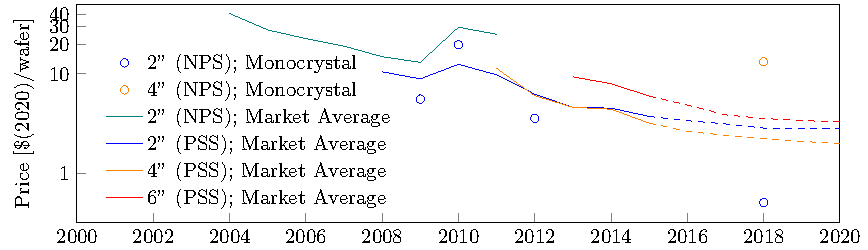
\includegraphics[width=15cm]{./figures/sapphire_prices.pdf}
    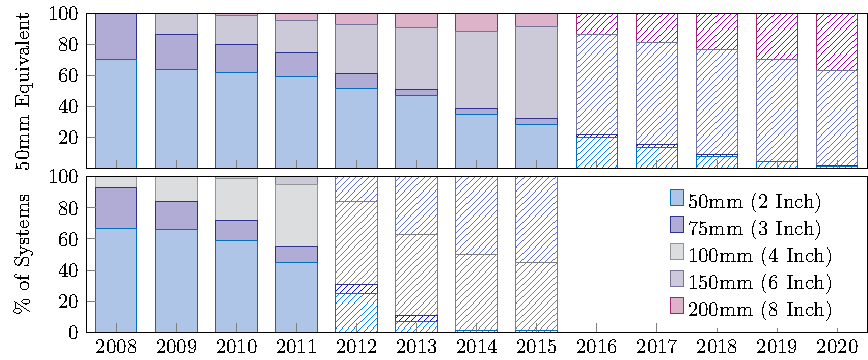
\includegraphics[width=14.5cm]{./figures/wafer_size.pdf}
	\caption{Top: Historical data for sapphire substrate prices of different surface properties and diameters. Shown is data for polished surface (NPS) and patterned substrates (PSS). \textit{Monocrystal} denotes the Russian manufacturer of the same name. Dashed lines are projections from the previous year. Sources: \cite{monocrystal2020private}\cite{yole2011sapphire}\cite{yole2015sapphire}. Bottom: Prevalence of sapphire wafer size used in the manufacturing of light-emitting diodes. Hatched bars are projections given by the sources. Sources: \cite{veeco2013}\cite{Scholand2012}\cite{yole2015sapphire}}
	\label{fig:wafers}
\end{figure}

\subsection{Preliminary Sensitivity Analysis}

\begin{figure}[h]
	\centering
    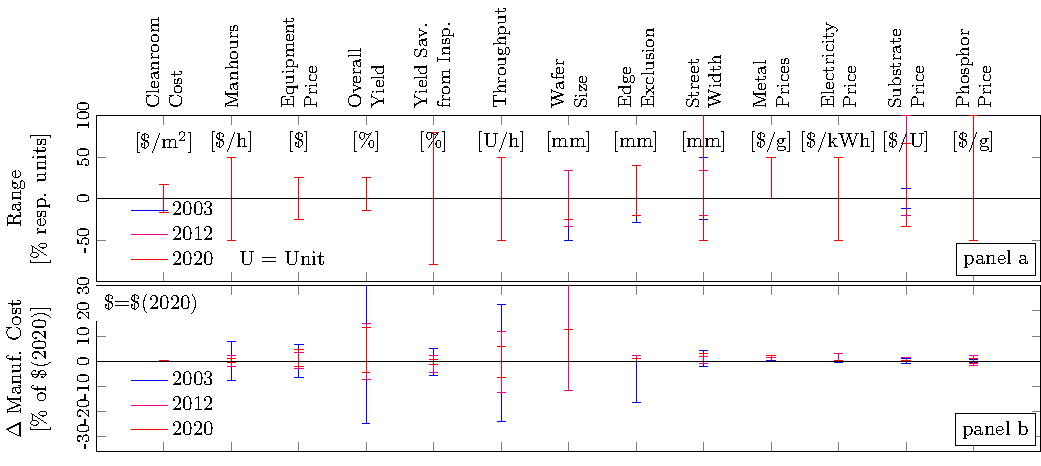
\includegraphics[width=\textwidth]{2_SSL_EES/article/figures/costmodel_sensitivity.pdf}
	\caption{Sensitivity analysis of selected cost model parameters. Note the decreasing sensitivity to cost model parameters as the number of die per wafer increases. Compare table \cref{tab:sensitivity}. Abbreviations: resp. - respective}
	\label{fig:sensitivity}
\end{figure}

A sensitivity analysis of the cost model has been performed using parameter variations listed in table \cref{tab:sensitivity}. The amount of parameter variation was chosen to encompass the identified range of the value of the parameter in different manufacturing setups of each considered year. As an example, the lower range in the variation for metal cost (+50\%,-0\%) was chosen because the metal prices in the model are price quotes from the United State Geological Survey price database. Industry metals are not sold below the price of the raw material and often the markup is small compared to the price of the material. The upper range was chosen, because a survey of industrial metal suppliers for semiconductor manufacturing showed that the largest markup was below 50\%. The results of the analysis are shown in  \cref{fig:sensitivity}. The cost model is generally more sensitive to variation of parameters at smaller wafer diameters. The most sensitive parameters are global parameters, such as yield or average equipment throughput.

\begin{table}[H]
\small
    \begin{tabularx}{\textwidth}{ |X|l|l|l|l|l|l|l|X|}
        \hline
            \textit{Parameter} & \textit{Unit} & \textit{2003} & $\pm [\%]$ & \textit{2012} & $\pm [\%]$ & \textit{2020} & $\pm [\%]$ & \textit{Source} \\
        \hline
            Cleanroom Cost & \text{USD}/m$^2$ & 3000 & +16,-16 & 3000 & +16,-16 & 3000 & +16,-16 & Figure \cref{fig:electricity+cleanroom_prices} \\
        \hline
            Manhours & FTE & 100\% & +50,-50 & 100\% & +50,-50 & 100\% & +50,-50 & I \\
        \hline
            Equip. Discount & \% of \text{USD} & 0\% & +25,-25 & 0\% & +25,-25 & 0\% & +25,-25 & I, \cite{Appleyard2001} \\
        \hline
            Overall Yield & \% & 100\% & +25,-25 & 100\% & +25,-15 & 100\% & +25,-25 & I, \cite{lumi2012yield}\cite{ledsmag2012} \newline \cite{systemplus2015reverse}\cite{ledcomv2} \\
        \hline
            Inspec. Yield Savings & \%/inspec. & 0.5\% & +80,-80 & 0.5\% & +80,-80 & 0.5\% & +80,-80 & \cite{mckinseyyield} \\
        \hline
            Overall Throughput & UPH or h$^{-1}$ & 100\% & +50,-50 & 100\% & +50,-50 & 100\% & +50,-50 & Datasheets \\
        \hline
            Wafer Diameter & mm & 100 & +0,-50 & 150 & +33.3,-33.3 & 200 & +0,-25 & I, Figure \cref{fig:wafer_size} \\
        \hline
            Edge Exclusion & mm & 7 & +0,-50 & 5 & +40,-0 & 5 & +40,-20 & \cite{ledsmagexclusion}\cite{rubiconexclusion} \newline \cite{xiamenexclusion}\cite{american2007annual} \\
        \hline
            Cutting Width & $\mu$m & 100 & +50,-25 & 75 & +33.3,-20 & 20 & +300,-50 & \cite{masaki2000division}\cite{ils2005width} \newline \cite{photonics2010width}\cite{discowidth} \\
        \hline
            Metal Prices & \text{USD}/kg & 100\% & +50,-0 & 100\% & +50,-0 & 100\% & +50,-0 & Datasheets \\
        \hline
            Electricity Price & \text{USD}/kWh & 100\% & +50,-50 & 100\% & +50,-50 & 100\% & +50,-50 & \cite{eia2000electric}\cite{eia2019electric} \\
        \hline
            Saph. Subst. Price & \text{USD} & 40 & +12.5,-12.5 & 10 & +100,-20 & 3 & +66.6,-33.3 & Figure \cref{fig:sapphire_prices} \\
        \hline
            Phosphor Prices & \text{USD}/g & 100\% & +50,-50 & 150 & +0,-0 & 200 & +0,-0 & I, \cite{yole_phosphor_2012}\cite{yole2017phosphor} \\
        \hline
        \end{tabularx}
    \caption{Cost model sensitivity analysis parameter list. For the sensitivity analysis performed using these variables, see  \cref{fig:sensitivity}. Units for values in columns \textit{2002}-\textit{2020} are indicated in column \textit{Units}. If values in columns \textit{2003}-\textit{2020} are instead are given in \%, this indicates that the parameters were varied by a set percentage from their respective model baselines.}
    \label{tab:sensitivity}
\end{table}

\subsection{Comparison with Reported Industry Data and DOE Projections}

We conducted a comparison of the LED manufacturing cost structure produced by our cost model with previously reported US DOE calculations and projections based on the LEDCOM model and industry data provided as part of industry round table discussions (see \cref{fig:costmodel_calibration}). We note some differences between the results of our model and the cost structure reported or projected by the DOE. For instance, the share of the epitaxy step is consistently larger in the DOE data. This can in part be explained by our model relying on state-of-the-art equipment at a virtual US-based manufacturing location, while industry might not run low-power and mid-power chip production on these, more expensive, reactors. In addition, the manufacturing lines of the majority of manufacturers is located in Asia. We also note that the share of the substrate price in the DOE data is much larger than in our model, which can in part be explained by the overestimation of the actual price of sapphire wafers in earlier projections for 2015-2020. Finally, the relative importance of the packaging part of the manufacturing process is very similar in our model and in the DOE results in 2012. However, in the DOE projections it significantly decreases by 2020, while in our model it retains and even increases its share of the total cost. This trend has been independently confirmed by researchers and industry reports on wafer-level packaging \cite{Lee2011WPL}\cite{Xie2013}\cite{ledsmag2017WLP}, showing better performance of our cost model compared to earlier DOE model projections

\begin{figure}[h]
	\centering
    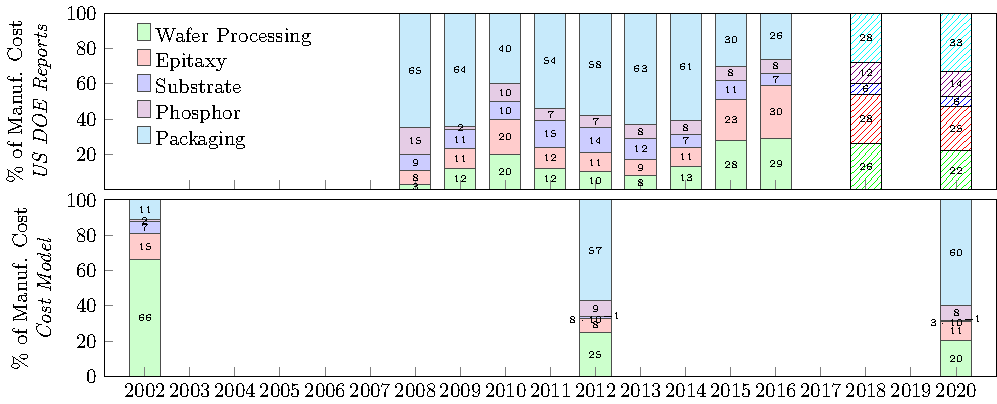
\includegraphics[width=\textwidth]{2_SSL_EES/article/figures/costmodel_calibration.pdf}
	\caption{Modelled manufacturing cost for light-emitting diode packages split by manufacturing step category. The top graph shows the data from LEDCOM model and round table discussions published by the United States Department of Energy (DoE). The bottom graph shows the results of the cost model developed in this thesis. Hatched bars are projections given by the sources. Inset plot shows the number of die per wafer (DPW) calculated for different wafer sizes used in the model. Sources for top panel: \cite{doe2010solid}\cite{doe2011solid}\cite{doe2012solid}\cite{doe2013solid}\cite{doe2014solid}\cite{doe2015solid}\cite{doe2016solid}. Sources for bottom panel: own elaboration based on the cost model described in Section \cref{sec:costmodel}. Sources for Inset Plot: own elaborations based on numerical approximations for die-per-wafer estimations provided in \cite{de2005investigation}, informed by expert interviews.}
	\label{fig:costmodel_calibration}
\end{figure}

\cref{fig:costmodel_calibration} shows a comparison of the relative manufacturing cost by manufacturing step categories between the cost model and data released by the United States Department of Energy (DoE). Note that any comparison between the s must consider: Our model assumes state-of-the-art equipment, while the DoE industry round table reports data from factories which use older equipment, as well as newer equipment. Our model presently considers only low-power and mid-power packages, while the DoE reports consider high-power packages also. Our model assumes a virtual North American manufacturing location, while the majority of manufacturers produce in Asia. We note that the share of the substrate price in the DoE data is much larger than in our model. This can in part be explained by  \cref{fig:sapphire_prices}, which already shows how projections overestimated the actual price for 2015-2020. We note also that the share of the epitaxy step is larger in the DoE model. This can in part be explained by our model relying on state-of-the-art equipment, while industry might not run low-power and mid-power chip production on these, more expensive, reactors. In conclusion, our model fits industry forecasts due to the way it is set up. The packaging part of the manufacturing process is increasing in importance, which has been confirmed by researchers and industry reports on WLP\cite{Lee2011WPL}\cite{Xie2013}\cite{ledsmag2017WLP}.

\section{Computation of Contribution of Individual Variables}

To quantify the drivers of cost reductions across all process steps, one would need to identify the magnitude of contribution to cost reductions made by single variables in equations \cref{eqn:cost_wafer} and \cref{eqn:cost_die}. Mathematically, given a function $C$ which describes the cost associated with manufacturing a single unit at time $t$,

\begin{myequation}
C=ab+cd
\end{myequation}

and manufacturing variables $a,b,c,d$, we are looking for the contribution $\Delta C_{a}$ made by a single variable $a$ to the total change in the cost function $\Delta C$ between points $t_0,t_1$ such, that

\begin{myequation}
\Delta C = C(t_1)-C(t_0) = \sum_{i=a, \dots, d} \Delta C_i
\end{myequation}

The infinitesimal contribution to the total cost by the infinitesimal change in a cost model variable is defined through the total differential of the cost function \cref{eqn:cost_sum} as

\begin{myequation}
\text{d}C(x_1 (t), x_2(t), \dots) = \sum_i \frac{\partial C }{\partial x_i}     \frac{\text{d}x_i}{\text{d}t} = \sum_i \frac{\partial C }{\partial x_i}  \Delta x_i
\end{myequation}

where $x_i$ is an arbitrary cost variable. The contribution of the change $\Delta x_1$ in variable $x_1$ to total cost $C$ over the period $t_0 < t < t_1 $ is then

\begin{myequation}
\Delta C_{x_1} = \int_{t=t_1}^{t_2} \frac{\partial C }{\partial x_1} \frac{\text{d}x_1}{\text{d}t} \text{d}t
\label{eqn:integral_1}
\end{myequation}

However, data on the cost model variables is not available in continuous time. Disaggregating the contribution of single variables to the total cost reduction is thus not straightforward in our model. This problem does not arise in cost models which compute cost changes directly, such as \cite{nemet2012solar} \cite{goodrich2013assessing}. The following discussion follows an approach developed by Kavlak et al. \cite{kavlak2018evaluating}. For the detailed derivation, we refer to this publication.

The cost function $C$ as a function of a vector of cost model variables $\vec{r}=(r_1,r_2,\dots)$ is defined as

\begin{myequation}
C(\vec{r}) = C(r_1,r_2, \dots) = \sum_i C_i
\end{myequation}

where

\begin{myequation}
C_i(\vec{r}) = C_i^0 \prod_w g_{iw}(r_w)
\end{myequation}

Using logarithmic differentiation, the integral from  \cref{eqn:integral_1} can be rewritten as

\begin{myequation}
\Delta C_x = \int_{t=t_0}^{t_1} C(t) \frac{ \partial \ln C }{ \partial x } \frac{ \text{d} x }{ \text{d} t} \text{d} t
\end{myequation}

where for $C(t)$ a constant $C(t) \approx \tilde{C} $ can be chosen such that $\Delta C_{x_i} = \Delta C$. In practice, this constant value can be approximated as $\tilde{C} \approx \frac{2}{3} C_i^\text{geo} + \frac{1}{3} \overline{C_i}$. The contribution of a single cost model variable $r_z$ can then be written as

\begin{myequation}
\Delta C_z (t_1,t_2) \approx \sum_i \tilde{C_i} \ln \frac{g_{iz}(t_2)}{g_{iz}(t_1)}
\end{myequation}

This approach was used to determine the effect of spillovers on device performance, displayed in  \cref{fig:breakthroughs_efficiency}. Due to time constraints, this approach could not be used to determine the effect of spillovers on manufacturing cost. Future work to quantify the impact of different cost drivers, including breakthroughs and changes in the manufacturing variables of  \cref{eqn:cost_sum}, could this method.

\section{Non-Phosphor-Related LED Innovations}

This section summarizes LED innovations and technology and manufacturing process improvements identified in this study as affecting key white LED sub-efficiencies, as discussed in section 5.1 and shown in Figures 4-6 in the main article. Note that phosphor-related LED innovations affecting consumer experience metrics, along with spectral efficiency, are presented separately in Table 1 in the main publication and discussed in detail in \cref{sec:innovation_phosphor}.

\begin{table}[H]
    \begin{tabularx}{\textwidth}{ |l|X|X|l|l| }
        \multicolumn{5}{c}{Forward Voltage Efficiency (VFE) $\eta_{Vf}$} \\
        \hline
            \textit{Year} & \textit{Innovation} & \textit{Area of Improvement} & \textit{Spillover} & \textit{Source} \\
        \hline
            1999 & Indium Tin Oxide \newline Current spreading layer & Contact resistance & Yes & \cite{margalith1999indium}\\
        \hline
            1998 & Digitated electrodes & Contact resistance & No & \cite{steigerwald2001electrode} \\
        \hline
            ongoing & Epitaxy improvements \newline and better doping & polarization and \newline bulk resistance & No & I \\
        \hline
            1998 & Silver p-Contacts & Contact resistance & No & \cite{kondoh2001nitride} \\
        \hline
        \multicolumn{5}{c}{Light extraction efficiency (LEE) $\eta_{LE}$} \\
        \hline
            \textit{Year} & \textit{Innovation} & \textit{Area of improvement} & \textit{Spillover} & \textit{Source} \\
        \hline
            $<$ 2003 & Optimization for \newline cavity effects & Other & No & I, \cite{Shen2003} \\
        \hline
            1993 & Chip surface randomization & Total reflection and absorption & No & I, \cite{bergh1973surface}\cite{Schnitzer1993} \\
        \hline
            1993 & Thin-film chip architecture & Absorption & No & I, \cite{Schnitzer1993} \\
        \hline
            1996 & Patterned sapphire substrate  & Total reflection and absorption & Yes & I, \cite{Tadatomo2001} \\
        \hline
            ongoing & Chip design for high LEE & Total reflection and absorption & No & I, \cite{Haerle2004} \\
        \hline
            $\sim$2000 & Silver p-contacts & Absorption & No & I, \cite{kondoh2001nitride} \\
        \hline
        \multicolumn{5}{c}{Internal quantum efficiency (IQE) $\eta_{IQ}$} \\
        \hline
            \textit{Year} & \textit{Innovation} & \textit{Area of improvement} & \textit{Spillover} & \textit{Source} \\
        \hline
            1994 & DH & Higher radiative recombination probability & No & \cite{Nakamura1994} \\
        \hline
            1996 & multiple quantum well & Higher radiative recombination probability & No & \cite{Koike1996} \\
        \hline
            ongoing & Active region \newline Doping & Both & No & I, \cite{schubert2018light} \\
        \hline
            ongoing & Epitaxy \newline Improvements & Both & No & I \\
        \hline
            ongoing & Chip architecture \newline Improvements & Both & No & I \\
        \hline
        \multicolumn{5}{c}{Light Conversion efficiency (CE) $\eta_{C}$} \\
        \hline
            \textit{Year} & \textit{Innovation} & \textit{Area of improvement} & \textit{Spillover} & \textit{Source} \\
        \hline
            ongoing & Lower current density & Current density & No & I \\
        \hline
            ongoing & Epitaxy \newline Improvements & Charge distribution \newline Defect density & No & I, \cite{bhardwaj2016progress} \\
        \hline
            ongoing & Chip architecture \newline improvements  & Charge distribution \newline Defect density & No & I, \cite{Wildeson2017} \\
        \hline
            $<$ 2017 & Defect getting \newline underlayer & Defect Density & No & I, \cite{haller2017burying} \\
        \hline
        \end{tabularx}
    \caption{LED innovations and technology improvements affecting key white LED device sub-efficiencies. The table includes innovations and technology improvements affecting forward voltage efficiency, light extraction efficiency, internal quantum efficiency, and light conversion efficiency. For a list of innovations affecting spectral efficiency, see Table 1 in the main article. Year column indicates the first instance of application of corresponding invention in white LEDs. Spillover column indicates if the innovation involved technology spillovers. Source column indicates the source of information about the innovation or improvement, with 'I' indicating expert interviews as such a source. Source column additionally indicates if the spillover has been identified as part of an expert interview (I).}
    \label{tab:innovations}
\end{table}

\section{Phosphor-Related LED Innovations}
\label{sec:innovation_phosphor}

This section provides additional details for phosphor-related LED innovations identified in this study as affecting both spectral sub-efficiences and consumer experience metrics and discussed in \cref{subsec:metrics}, Table 1 and Figures 5-7 in the main article. 

\subsection{History of Identified Phosphor-Related LED Innovations"}

\subsubsection{YAG and YGAG Phosphors}

Prior to Nakamura’s invention of highly efficient blue LEDs in the 1990s, Japan’s Nichia Corporation had not sold commercially successful semiconductor products, instead specializing in phosphors for cathode ray tubes (CRT) and fluorescent lamps \cite{nakamura2013blue}  . Nevertheless, extensive firm expertise in this area helped Nichia’s Yoshinori Shimizu formulate the principles of using CRT phosphors to convert blue light from Nakamura’s LEDs into white light in 1994 \cite{shimizu1994sheet}\cite{cho2017white}. By 1996, Shimizu and his colleagues developed \cite{bando1996}\cite{shimizu1999light} the first practical LED application of a well-known Yttrium Aluminium Garnet (YAG) CRT phosphor activated with cerium \cite{blasse1967new}, enabling the first commercial white LED products manufactured and sold by Nichia since late 1996 \cite{bando1998development}\cite{cho2017white}. 

Importantly, the YAG phosphor does not exhibit the spectral properties desirable in general illumination applications (see Figure 7 in the main article). An early solution to this problem, which was first discovered in the late 1967 \cite{holloway1969optical} and suggested for LEDs by the same team at Nichia in 1996 \cite{bando1998development}\cite{shimizu1999light}, was to use the gadolinium-doped red-shifted YAG phosphor (YGAG). Used in combination with red-emitting sulfide phosphors, by 2002 it helped bring to the market the first generation of warm white light LED products, e.g., those produced by Lumileds \cite{Mueller2002}. However, sulfide phosphors led to accelerated deterioration of sensitive parts of LED devices and became less efficient as operating temperatures increased. New chemically stable and non-toxic red phosphors were needed. 

\subsubsection{258, SLA and SALON phosphors}

In 1997, Hubert Huppertz and Wolfgang Schnick, working at the University of Bayreuth in Germany, synthesized the first compound in a new class of rare earth nitridosilicate materials \cite{Huppertz1997} later dubbed “258” due to a proportion of elements in its chemical formula. The luminescent properties of these materials were identified by the Schnick’s group, by then at Ludwig-Maximilians University of Munich, in 2000 \cite{Hppe2000} after a suggestion made to Schnick at a conference following earlier reports of good luminosity properties of europium-doped compounds \cite{Qiua1998}. U.S.-based LED manufacturer Lumileds applied for a patent for the first class of red LED phosphors based on the 258 nitridosilicate chemistry in 2002 \cite{mueller2004phosphor}. The first use of the 258 phosphor in a commercial “Luxeon” LED package was then reported in a joint publication co-authored by inventors from Lumileds and researchers from the Schnick’s group in 2005 \cite{MuellerMach2005}.

Further efforts in LED phosphor development were directed towards synthesizing a red narrow-band phosphor. Narrow LED emission peak widths yield the highest luminous efficacy of radiation, as in this case less light is emitted in the far-red range of the spectrum in which the human eye is not very sensitive. After synthesizing several narrow-band phosphors emitting in yellow \cite{Hppe2004} and cyan \cite{Kechele2009}, the Schnick’s group identified the local cubic cation coordination structure of the cyan phosphor compound as the reason for its narrow band width \cite{lumi2016narrow}. A search for a structurally analogous nitride compound with the narrow red instead of the cyan emission was undertaken. After several unsuccessful attempts, the sought-after cuboidal nitride compound was found in a 2008 publication led by Francis DiSalvo \cite{Park2008Sr}. Based on information provided in this work, Schnick and colleagues synthesized and studied the spectral properties of a new narrow band red SLA phosphor in 2013 \cite{schmidt2013new}\cite{Pust2014}\cite{schmidt2017phosphors}. The material was introduced in commercial LED devices by Lumileds in 2015 \cite{lumi2016narrow_whitepaper}. 

The most recent red narrow-band phosphor innovation included in Table 1 and Figure 7 in the main article, indicated as SALON, has been under development during the late 2010s by a group of Austrian and German researchers that included Huppertz, the discoverer of the “258” material, working in collaboration with Osram, another major LED manufacturer \cite{seibald2019phosphor}\cite{Hoerder2019}\cite{Hoerder2020}. The first patent application for this phosphor was filed in 2016 . The SALON phosphor is a derivate of the SLA phosphor. Therefore, it is the only innovation related to consumer experience metrics identified in our study that seemingly not involved technology spillovers.

\subsubsection{PFS Phosphor}

Down conversion with ultra-narrow-band phosphor can achieve the highest spectral efficiency. However, few such phosphors have been identified, with even less exhibiting desirable material properties such as thermal stability \cite{Phillips2007}. The first commercially successful ultra-narrow-band red phosphor was developed by General Electric (GE). It is based on a potassium fluorosilicate (PFS) compound activated with manganese ions. Its luminescence was first recorded by Adrian Paulusz at GE in 1972 \cite{paulusz1973efficient}. In the early 2000s, while searching for potential new LED phosphor materials for GE’s lighting business at GE Lumination, Emil Radkov rediscovered Paulusz’s findings in the literature. Following extensive research on PFS chemical synthesis and material properties conducted in collaboration with the University of Sofia in Bulgaria, Radkov’s Alma Mater, the PFS phosphor had been under development at GE since 2005 \cite{radkov2006red}\cite{radkov2009red}. This work, supported by public funding from the U.S. Department of Energy (DOE) Solid-State Lighting program \cite{doesslprogram}, resulted in a series of critical improvements in the PFS phosphor properties \cite{Setlur2010}\cite{lyons2012color}, eventually enabling its commercialization under the “TriGain” brand in 2015 \cite{trigain_spectrum}\cite{setlur2015trigain}\cite{Murphy2015}.

\subsubsection{Quantum Dots for Light Down-Conversion}

Quantum dots (QD) are semiconductor nanocrystals whose quantum size effects make QDs behave as “artificial atoms”. Semiconductor quantum dots were first synthesized in the Soviet Union in 1981 \cite{ekimov1981quantum} and at Bell Labs in the U.S. in 1983 \cite{Rossetti1983}. Luminescent properties of quantum dots were first empirically observed in 1984 \cite{fojtik1984photo} and extensively studied in the early 1990s. The key feature of QD luminescence discovered in those studies is that its colour is determined by the QD particle size, making it possible to create pure monochromatic blue, green and red light sources just by tuning the QD size. The first application of QDs in LEDs was reported in 1994 in an electroluminescent hybrid QD-polymer LED. However, this LED type could not be used in general illumination due to its very low luminous efficacy. An alternative application of QDs as a kind of a “phosphor” for light down conversion from an LED light source was proposed in the early 2000s as part of the U.S. Department of Energy (DOE)-funded “A Revolution in Lighting“ project at Sandia National Laboratory \cite{simmonsfinal}. This concept was successfully demonstrated by Sandia researchers on a commercial LED in 2003 \cite{shea_rohwer_development_2004}\cite{noauthor_sandia_nodate} and was swiftly taken up and advanced further by a group in Taiwan \cite{Chen_2005}\cite{Hsueh_Shih_Chen_2006} The first commercial application of QDs in an LED lamp was brought about by a collaboration between an MIT-born startup QD Vision and the U.S.-based luminaire manufacturer Nexxus Lighting in 2009 \cite{ledprof_nexxusqd}, \cite{bourzac2013quantum}. However, rapid advances in the spectral and conversion performance of down-conversion phosphors and high manufacturing cost of quantum dots resulted in the discontinuation of this product. After finding market success in display backlighting first demonstrated by Samsung in 2010 \cite{Jang2010} and commercialized by QD Vision in Sony television sets in 2013 \cite{bourzac2013quantum}, QDs returned to the general lighting market in products offered by Lumileds \cite{noauthor_global_2017}\cite{noauthor_quantum_2020} around 2017 and Osram in 2019 \cite{osramqdots} in the form of mid-power LED packages that combined QDs with traditional phosphors for light down conversion.

\subsection{Spectral Data for Identified LED Phosphor Innovations}

\begin{figure}[H]
	\centering
    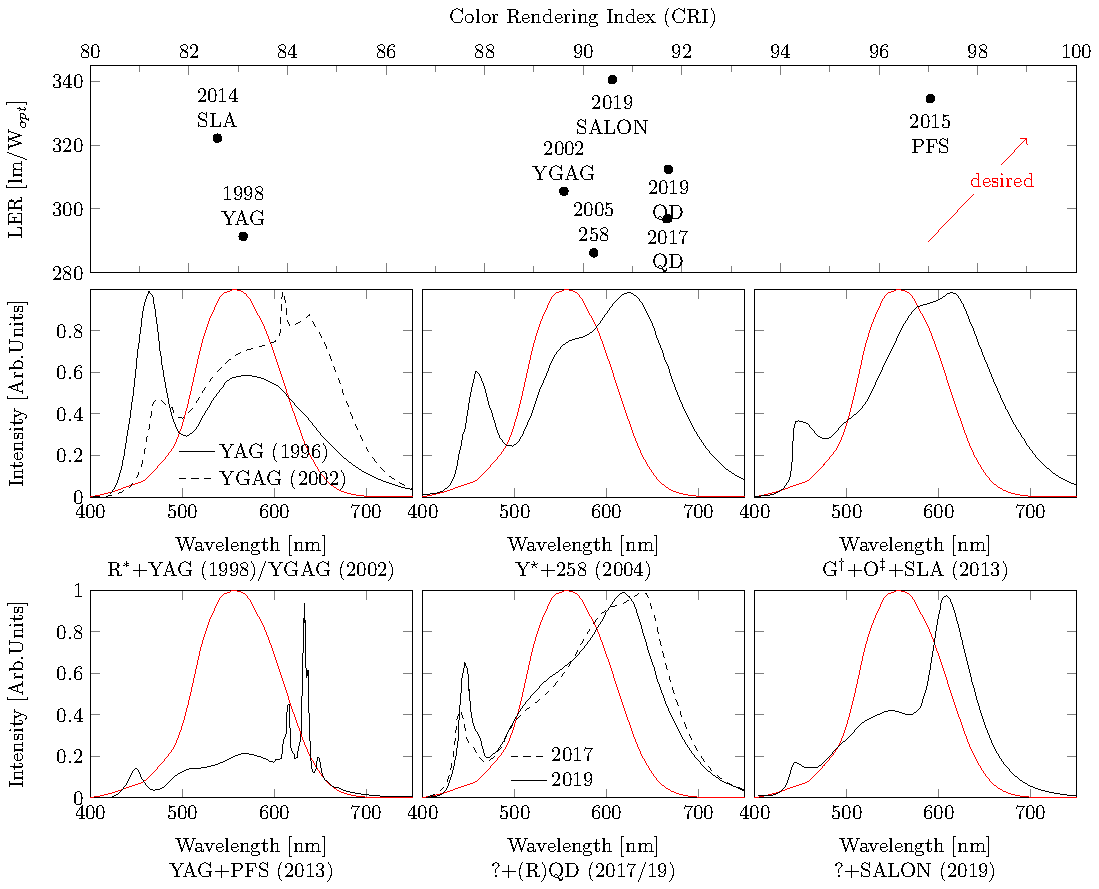
\includegraphics[width=0.95\textwidth]{2_SSL_EES/article/figures/phosphor_spectrum-comparison.pdf}
	\caption{Spectral data and additional consumer experience metrics for the earliest identified representative white LED products with published spectral data, shown in Figure 7 in the main article, that used phosphor innovations listed in Table 1 in the main article, each indicated by the phosphor label and spectral data publication year. Top panel: Luminous efficacy of radiation (LER) and colour rendering index (CRI) of white LED devices represented in Figure 7 in the main article. The desirable direction of improvements towards higher luminous efficacy at higher CRI is indicated by a red arrow. Metrics were calculated from spectral data shown in the two bottom panels using the \texttt{colour-science} package for Python \cite{colour-science_software}. Bottom two rows of panels: Corresponding spectral data. The luminosity function \cite{cie-term-lumeff}, describing the wavelength-dependent sensitivity of the human eye, is shown for reference in red in each panel. Note that peaks or large tails of the device emission spectrum at the far ends of the luminosity function are not desirable, as the photons of the corresponding energy are lost to the human eye and count towards the spectral loss channel.  Abbreviations: Arb. Units - Arbitrary Units (compare section \cref{subsec:arbunit}). Plot legends indicate the years of publication of the spectral data and phosphor mixtures used in corresponding LED devices, with the following designations for additional phosphor mix components: O$^\ddagger$ -  other parts of phosphor mixture not disclosed, G$^*$ - \ch{CaSrS:Eu^{2+}}, Y$^\star$ - $\beta-$SiAlON:Eu$^{2+}$, $^\dagger$ - \ch{Lu_3Al_5O_{12}:Ce^{3+}}, $^\ddagger$ - \ch{(Ba,Sr)_2Si_5N_8:Eu^{2+}}. Source (top panel): own elaboration based on spectral data. Arb. Units - Arbitrary Units, defined as the ratio of radiation intensity at a wavelength compared to the highest point in the spectrum. Sources: top panel - own elaboration based on spectral data; bottom two panels: adapted from published spectral data for LEDs with the following phosphors: YAG \cite{bando1998development}, YGAG \cite{Mueller2002}, 258 \cite{MuellerMach2005}, SLA \cite{Pust2014}, PFS \cite{trigain_spectrum}, QD \cite{lumileds2016qd}\cite{osram2019qd}, SALON \cite{Hoerder2019}.}
\label{fig:phosphor_spectrum}
\end{figure}

\section{List of Interviewees}

\begin{table}[h!]
\small
    \centering
    \begin{tabular}{|l|l|l|l|l|}
    \hline
        \textit{\#} & \textit{Sector} & \textit{Role} & \textit{Country} & \textit{Expertise} \\ \hline
        1 & Academia & Sr. researcher & UK & Epitaxy \\ \hline
        2 & Industry & Consultant, former sr. researcher & USA & Device architecture \\ \hline
        3 & Industry & Consultant, former head of R\&D & Germany & Epitaxy \\ \hline
        4 & Academia & Professor & Austria & Phosphors \\ \hline
        5 & Industry & Consultant, former head of R\&D & USA & Device architecture \\ \hline
        6 & consulting & Consultant, former sr. technical advisor & USA & Device architecture \\ \hline
        7 & Academia & Professor & Germany & Phosphors \\ \hline
        8 & government & R\&D manager & USA & Device architecture \\ \hline
        9 & consulting & Consultant & USA & Device applications \\ \hline
        10 & Academia & Professor & France & Device physics \\ \hline
        11 & Industry & Sr scientist, former head of R\&D & USA & Device architecture \\ \hline
        12 & Industry & Principal scientist & Germany & Phosphors \\ \hline
        13 & Industry & Former head of R\&D & USA & Phosphors \\ \hline
    \end{tabular}
    \label{tab:interviews}
    \caption{Anonymized list of LED experts interviewed for this study. Abbreviations: sr. - senior}
\end{table}

\clearpage
\newpage
\section{Complete List of Sources for Figures}
\label{sec:sources}

\subsection{Figure 1 (Historical Development of Luminous Efficacy)}

The list of sources for Figure 1 in the main article is organized by different technologies:

\begin{table}[h!]
    \begin{tabularx}{\textwidth}{|l|X|}
    \hline
    \textbf{Technology} & \textbf{References} \\
    \hline
    LED & own research, compare \cite{zenodo_weinold_led_history} \\
    \hline
    CFL (<1984) & \cite{Bouwknegt1982}\cite{Vrenken1983} \\
    \hline
    CFL (1984-2011) & \cite{eger2018origin} \\
    \hline
    CFL (>2011) & \cite{Guan2015} \\
    \hline
    Fire, Incandescent, HID & \cite{azevedo2009transition} augmented by own calculations based on \cite{benesch1905beleuchtungswesen} \\
    \hline
    Max. efficacy & \cite{Murphy2012} \\
    \hline
    \end{tabularx}
\end{table}

\subsection{Figure 2 (Historical Development of Lamp Prices)}

The sources for Figure 2 in the main article are grouped by the provider of data:

\begin{table}[h!]
    \begin{tabularx}{\textwidth}{|l|X|}
    \hline
    \textbf{Provider of References} & \textbf{References} \\
    \hline
    Stiftung Warentest (Germany) & \cite{Warentest2008}\cite{Warentest2009_1}\cite{Warentest2009_2}\cite{Warentest2010_1}\cite{Warentest2010_2}\cite{Warentest2011}\cite{Warentest2012}\cite{Warentest2013}\cite{Warentest2014_1}\cite{Warentest2014_2}\cite{Warentest2015}\cite{Warentest2016_1}\cite{Warentest2016_2}\cite{Warentest2018} \\
    \hline
    Konsument (Austria) & \cite{Konsument2010} \\
    \hline
    Which (UK) & \cite{Which2020} \\
    \hline
    Industry Periodicals & \cite{PM2020} \\
    \hline
    Government Reports & \cite{council2013assessment} \\
    \hline
    \end{tabularx}
\end{table}

\subsection{Figure 3 (Historical Evolution of LED Chip Architectures)}

The sources for Figure 3 in the main article are grouped by their type:

\begin{table}[h!]
    \begin{tabularx}{\textwidth}{|l|X|}
    \hline
    \textbf{Type of Source} & \textbf{References} \\
    \hline
    Scientific Publications & \cite{plossl2010wafer}\cite{bierhuizen2007performance}\cite{gencc2019distributed}\cite{chong2014performance} \\
    \hline
    Patents & \href{https://worldwide.espacenet.com/patent/search?q=pn\%3DJPH11168235A}{JPH11168235A}, 
\href{https://worldwide.espacenet.com/patent/search?q=pn\%3DDE19921987A1}{DE19921987A1}, 
\href{https://worldwide.espacenet.com/patent/search?q=pn\%3DJPH11340514A}{JPH11340514A}, 
\href{https://worldwide.espacenet.com/patent/search?q=pn\%3DJP2001044498A}{JP2001044498A}, 
\href{https://worldwide.espacenet.com/patent/search?q=pn\%3DUS2005045893A1}{US2005045893A1}, 
\href{https://worldwide.espacenet.com/patent/search?q=pn\%3DUS2002093023A1}{US2002093023A1}, 
\href{https://worldwide.espacenet.com/patent/search?q=pn\%3DUS2006273339A1}{US2006273339A1}  \\
    \hline
    Other Publications & \href{https://web.archive.org/web/20170801160530/https://www.energy.gov/sites/prod/files/2015/02/f19/craford_innovation_sanfrancisco2015.pdf}{2015 presentation (www.energy.gov)} \newline
\href{https://web.archive.org/web/20170715230721/https://www.energy.gov/sites/prod/files/2016/02/f29/sun_china_raleigh2016.pdf}{2016 presentation (www.energy.gov)} \newline
\href{http://web.archive.org/web/20160425025936/https://www.slideshare.net/Yole_Developpement/yole-led-packagingjanuary2013reportsample}{2013 presentation (www.slideshare.net)} \\
    \hline
    \end{tabularx}
\end{table}

\subsection{Figure 4 (Historical Developments in Device Sub-Efficiencies)}

The sources for Figure 4 in the main article are grouped by sub-efficiencies represented on different panels of the figure:

\begin{table}[h!]
    \begin{tabularx}{\textwidth}{|l|X|}
    \hline
    \textbf{Panel (Sub-Eff.)} & \textbf{References} \\
    \hline
    Panel A1 ($V_f$) & \cite{nichia2001data}\cite{lumi2002data}\cite{gen2005data}\cite{candlepwr2005data}\cite{lumi2006data}\cite{lumi2007data}\cite{nichia2008data}\cite{lumi2008data}\cite{osram2008data}\cite{jeong2011high}\cite{osram2012data}\cite{osram2013data}\cite{osram2014data} \newline \cite{lumi2016data_1}\cite{lumi2016data_2}\cite{epistar2017data}\cite{osram2017data_1}\cite{osram2017data_2}\cite{samsung2017data}\cite{samsung2018data}\cite{osram2018data}\cite{epistar2018data}\cite{lumi2019data} \\
    \hline
    Panel A2 (Droop) & Data calculated from luminous intensity curves of respective device datasheets: \cite{datasheet_osram_topled}\cite{osram2008data}\cite{osram2008gdplus}\cite{osram2018csp}\cite{datasheet_lumileds_lux1}\cite{lumi2008data}\cite{lumi2016data_1}\cite{lumi2016data_2}\cite{samsung2018data} \\
    \hline
    Panel B1 (IQE) & own research, compare \cite{zenodo_weinold_led_history} \newline
\cite{doe_ssl_multiyear_2006}\cite{doe_ssl_multiyear_2007}\cite{doe_ssl_multiyear_2008}\cite{doe_ssl_multiyear_2009}\cite{doe_ssl_multiyear_2010}\cite{doe_ssl_multiyear_2011}\cite{doe_ssl_multiyear_2012}\cite{doe_ssl_multiyear_2013}\cite{doe_ssl_multiyear_2014}\cite{doe_ssl_rnd_2015}\cite{doe_ssl_rnd_2016} \\
    \hline
    Panel B2 (LEE) & \cite{lee2005analysis}\cite{krames2007status}\cite{Jang2004}\cite{Horng2013}\cite{Liao2010}\cite{HungWenHuang2005}\cite{Leem2007}\cite{Huang2008}\cite{Wang2009}\cite{Huh2003}\cite{Horng2008}\cite{Gao2008}\cite{Chang2003}\cite{Zhou2012} \newline \cite{ChunJuTun2006}\cite{Hua2009}\cite{Matioli2010}
\cite{lee2005analysis}\cite{Zhu2015}\cite{Ding2015}\cite{Taki2019}\cite{Shchekin2006}\cite{Hu2016}\cite{Horng2010}\cite{Lin2016}\cite{Yue2018}\cite{Zhao2012}\cite{Zhu2015}\newline \cite{Ding2015}\cite{wierer2001high}\cite{Steigerwald2002}\cite{DaeSeobHan2006}\cite{Wang2006}\cite{Lee2007}\cite{Shen2007}\cite{Huang2006}\cite{Zhmakin2011} \\
    \hline
    \end{tabularx}
\end{table}

\newpage
\bibliographystyle{IEEEtran}
\bibliography{bibliography}

\end{document}
